% AJ,APJ copyright persmissions: https://journals.aas.org/article-charges-and-copyright/#AAS_material
% MNRAS copyright permissions https://academic.oup.com/mnras/pages/rights_and_new_business_development
% A&A email to (e-mail: aanda.paris@obspm.fr) 

%%%%%%%%%%%%%%%%%%%% author.tex %%%%%%%%%%%%%%%%%%%%%%%%%%%%%%%%%%%
%
% Template for the Handbook of X-ray and Gamma-ray Astrophysics (preliminary version)
%
%%%%%%%%%%%%%%%% Springer %%%%%%%%%%%%%%%%%%%%%%%%%%%%%%%%%%
\documentclass[graybox, nosecnum]{svmult}

% choose options for [] as required from the list
% in the Reference Guide

\usepackage{mathptmx}       % selects Times Roman as basic font
\usepackage{helvet}         % selects Helvetica as sans-serif font
\usepackage{courier}        % selects Courier as typewriter font
\usepackage{type1cm}        % activate if the above 3 fonts are
                            % not available on your system
%
\usepackage{makeidx}         % allows index generation
\usepackage{graphicx}        % standard LaTeX graphics tool
                             % when including figure files
\usepackage{multicol}        % used for the two-column index
\usepackage[bottom]{footmisc}% places footnotes at page bottom
\usepackage{hyperref}        %for hyperlinks
\usepackage{soul}            % for high-lighting of text
\hypersetup{colorlinks=true,urlcolor=blue}
%
\usepackage[square,numbers]{natbib}
%\bibliographystyle{ieeetr}
\newcommand{\hbindex}[1]{\hl{#1}\index{#1}}  %highlights index entries
\makeindex             % used for the subject index
                       % please use the style svind.ist with
                       % your makeindex program
%%%%%%%%%%%%%%%%%%%%%%%%%%%%%%%%%%%%%%%%%%%%%%%%%%%%%%%%%%%%%%%%%%%%%%%%%%%%%%%%%%%%%%%%%

\begin{document}
%\tableofcontents{}
\title*{Pre main sequence:  Accretion \& Outflows}
% Use \titlerunning{Short Title} for an abbreviated version of
% your contribution title if the original one is too long
\author{Christian P. Schneider  \thanks{corresponding author}, H. Moritz G\"unther and S. Ustamujic}
% Use \authorrunning{Short Title} for an abbreviated version of
% your contribution title if the original one is too long
\institute{Christian P. Schneider \at Hamburg Observatory, Gojenbergsweg 11, 21029 Hamburg, Germany, \email{christian.schneider@hs.uni-hamburg.de}
\and H. Moritz G\"unther \at Kavli Institute for Astrophysics and Space Research, Massachusetts Institute of Technology,
77 Massachusetts Avenue, Cambridge, MA 02139, USA \email{hgunther@mit.edu}
\and S. Ustamujic \at Institute 2, Address of Institute 2 \email{sabina.ustamujic@inaf.it}}
%
% Use the package "url.sty" to avoid
% problems with special characters
% used in your e-mail or web address
%
\maketitle
%
\abstract{Each chapter should be preceded by an abstract (about 250 words) that summarizes the content. The abstract will appear \textit{online} at \url{www.SpringerLink.com} and be available with unrestricted access. This allows unregistered users to read the abstract as a teaser for the complete chapter. Please do not include reference citations, cross-references or undefined abbreviations in the abstract.}
\section{Keywords}
Please provide keywords required to facilitate search of chapter on web; maximum 10 keywords.


\section{Introduction {\normalfont (3 pages) [Christian]}}

``The fundamental problem of star formation is how stars accrete their mass.'' \citep{Dunham_2014}.


How did the Sun form, how the Earth? Answering these questions requires the identification and study of the Sun's progenitors,  young stellar objects that will evolve into a stellar system like ours. Therefore, we primarily discuss stars and system s broadly resembling the young Sun, i.e., with masses below about 2$\,M_\odot$.

Such stars and planets form in molecular clouds, often associated with filaments within the clouds,  where denser, cooler parts collapse. In these regions, gravity dominates over the stabilizing effects of thermal pressure, turbulence, and magnetic fields \citep[e.g., ][]{McKee_2007} and protostars form  \citep{Andre_2014}. The first, self-gravitating, hydrostatic core contains only a small fraction of the final stellar mass ($\sim0.01\,M_\odot$) and most of the mass still in the envelope \citep[e.g.,][]{Gong_2015,Lee_2020}; these objects are called class~0 objects \citep[see Fig.~\ref{fig:starform_classes} top left, and ][]{Andre_1993, Larson_2003}. Due to angular momentum conservation, a disk forms around the central condensation and outflows are launched, which regulate the angular momentum balance of the system. The collimated outflows, jets, propagate into the interstellar medium beyond the envelope and are often the first detectable signs of a forming star. After disk formation, accretion proceeds through the disk onto the protostar. Eventually, the protostar's mass equals the envelope mass after roughly $10^5$\,yrs and the objects are called class~{\sc i} objects (Fig.~\ref{fig:starform_classes} top right), they are also hotter and more luminous than class~0 objects.

Eventually, the envelope disperses and the young stellar object (YSO) becomes visible at optical wavelengths at a stellar age of $\sim1\,$Myr. The dispersal mechanism is not clear yet, but winds and radiation from nearby OB stars if present or otherwise radiation and outflows from low mass stars likely play a major role. Also the (wide-angle) winds launched by the forming stellar system itself may contribute to the envelope dispersal and to reduce the envelope to star mass conversion efficiency of to one third \citep{Frank_2014}. Accretion then proceeds from the disk in these class~{\sc ii} sources or classical T~Tauri stars. It is this stage of star formation, where we first get a relatively unobscured view to the newborn stars (Fig.~\ref{fig:starform_classes} bottom left).

\begin{figure}[t]
\centering
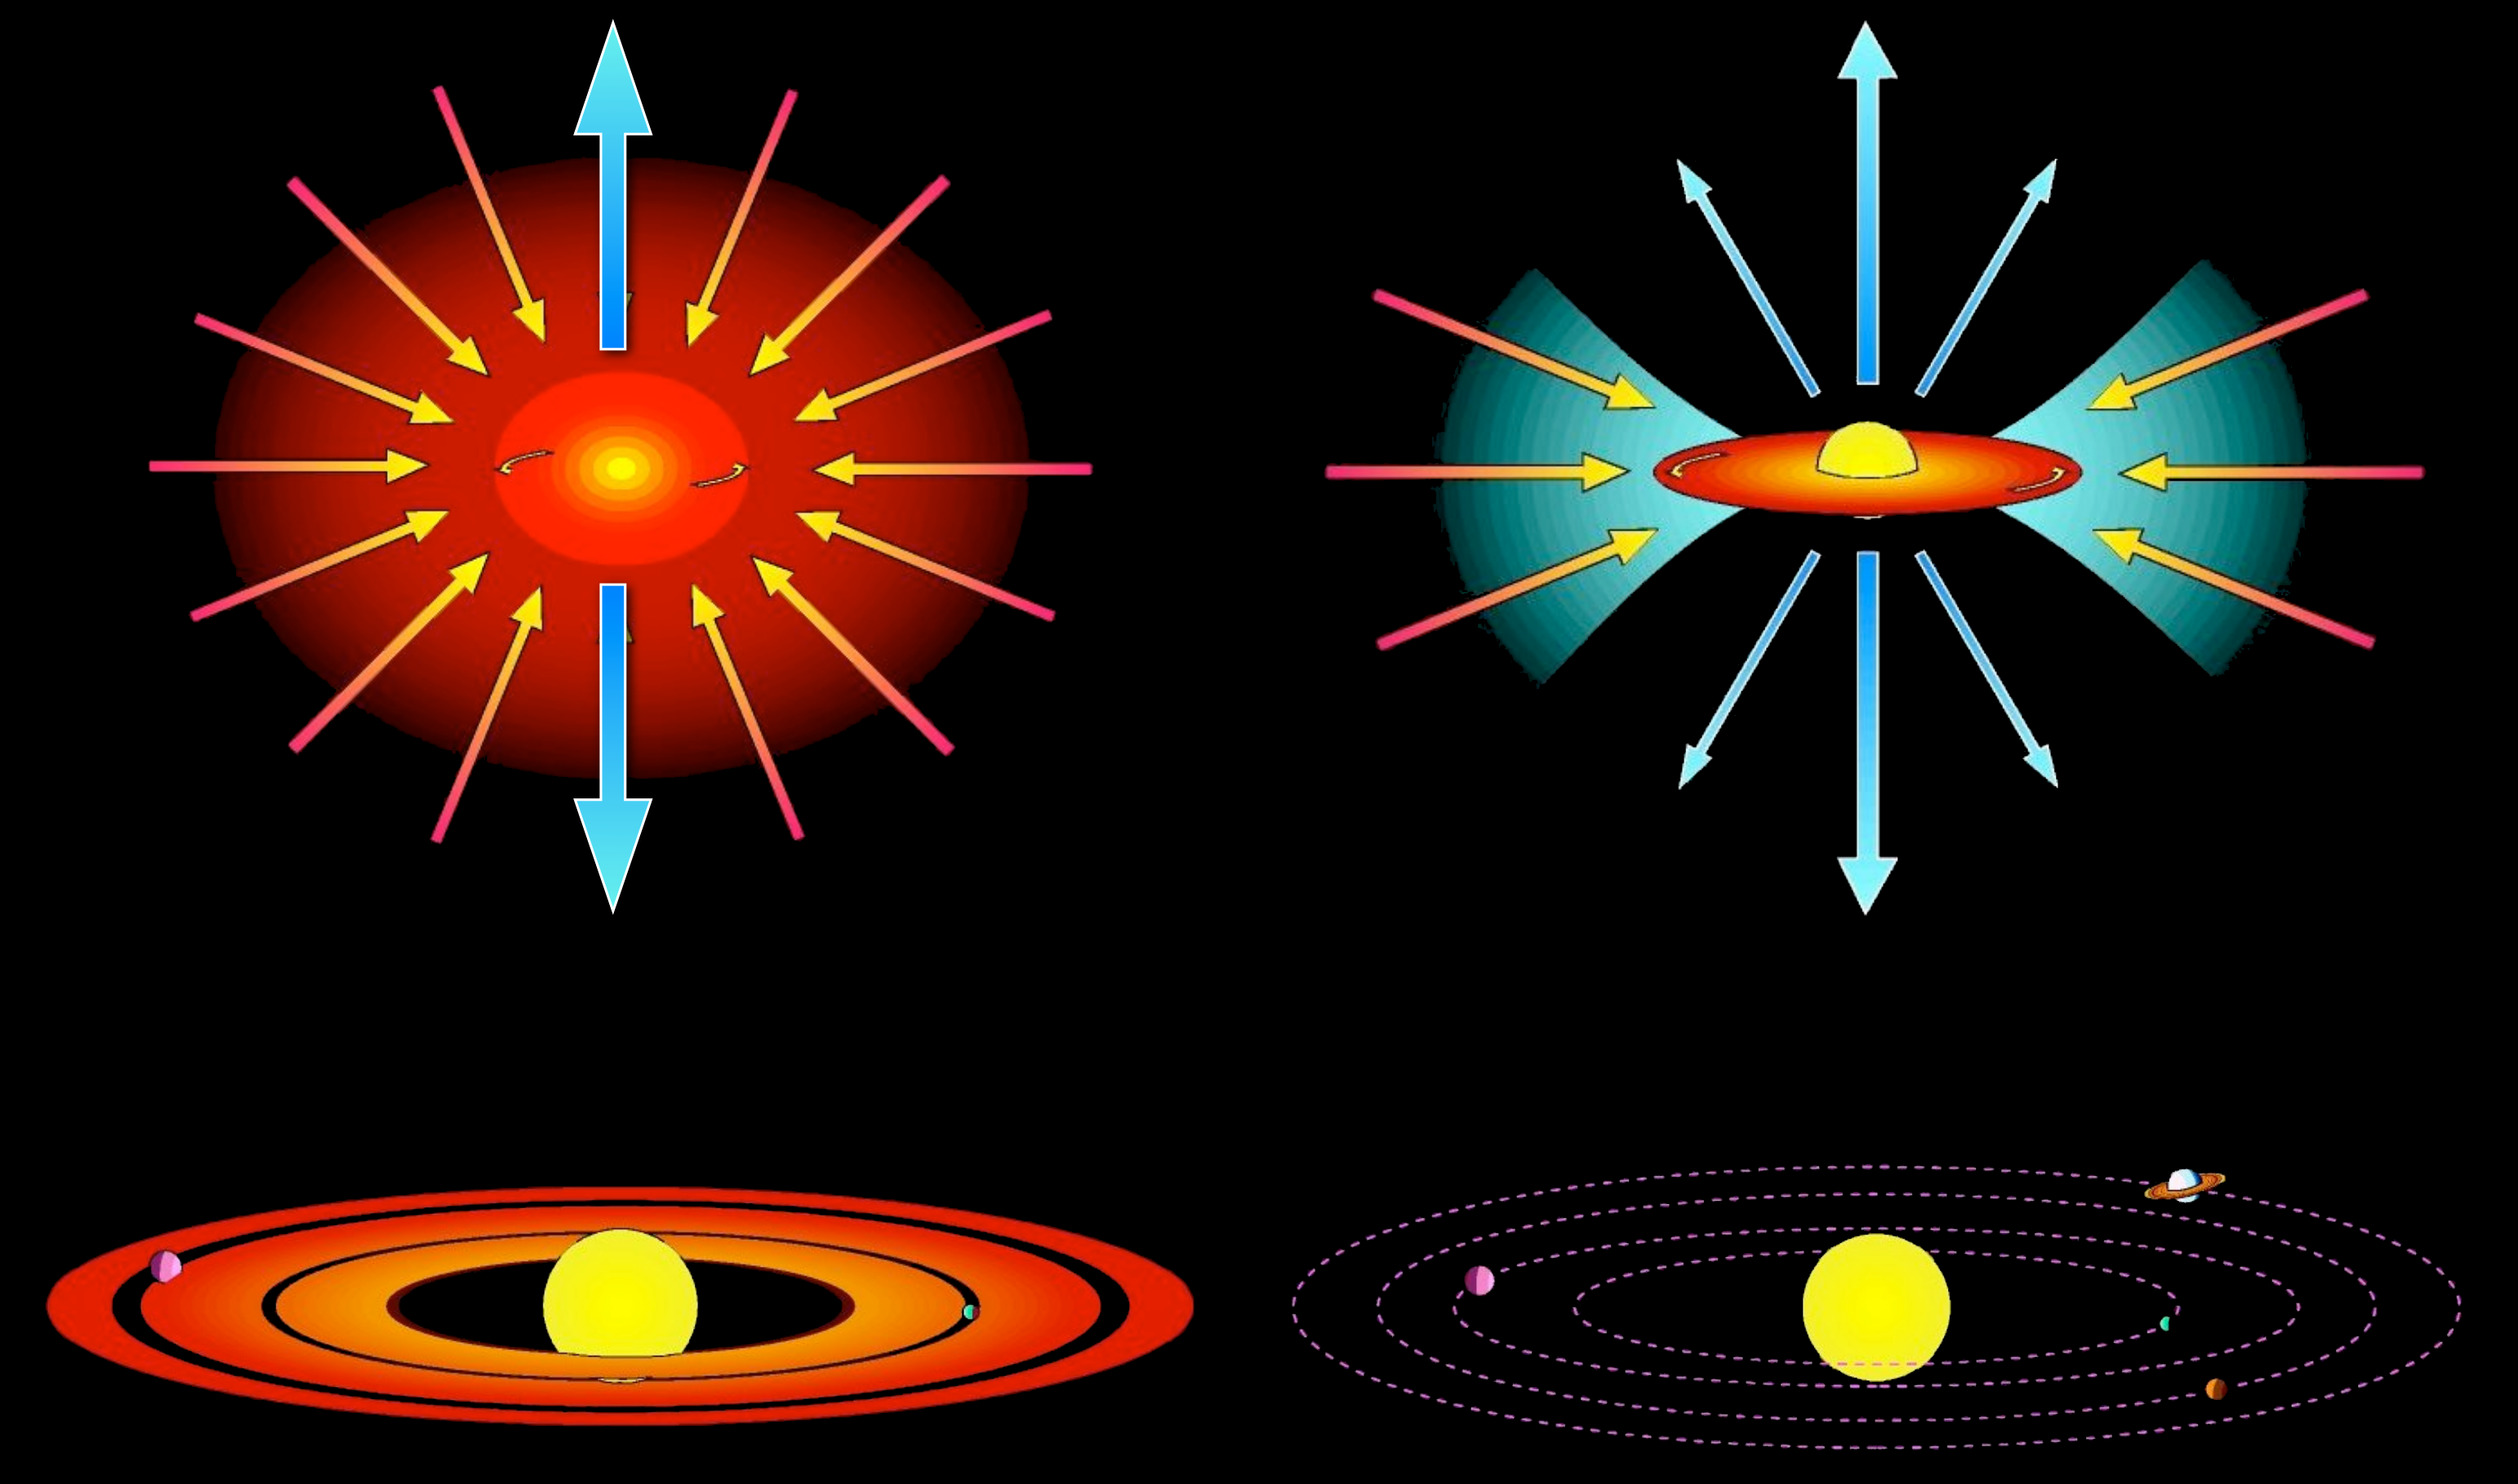
\includegraphics[width=10cm]{figs/starform_classes.png}
\caption{Star formation sequence. Adapted from original diagram by M.~McCaughrean. \label{fig:starform_classes}}
\end{figure}

Finally, the disk dispersed, too, after another few Myrs leaving behind a pre-main sequence star, perhaps surrounded by planetary system, which slowly contracts towards it's  main-sequence radius (Fig.~\ref{fig:starform_classes} bottom right). Solar mass stars take approximately 100\,Myrs to reach the main sequence where they reside for over 10\,Gyr.

Within this sequence of star formation, the classical T~Tauri star phase stands out, because the relatively unobscured view towards the central region around the forming stars provides us with the most detailed picture of the physical processes, including planet formation, using a large variety of observational techniques including X-ray data.

\subsection{T Tauri Stars}
T~Tauri stars as a distinct class of objects were first described by \citeauthor{Joy_1945} in 1945 based on their pronounced optical variability \citep{Joy_1945}. The notation that T~Tauri stars are young came with the realization that they are located to the top right of  main sequence (MS) stars in the Hertzsprung-Russel diagram (HRD), consistent with the expected position of stars contracting along their Hayashi tracks towards the MS \citep{Hayashi_1961}. Also, strong Li absorption lines suggest a young age, because  Li is quickly depleted in stellar photospheres \citep{Magazzu_1992}.

The physical processes that cause other prominent features seen in CTTSs remained controversial. For example, there was consensus on the origin of the
strong emission lines like H$\alpha$, termed “chromospheric emission”, until the 1980s. When the infrared excess of CTTSs was discovered and correctly ascribed to cold dusty disks around the central star and the ``chromospheric'' line profiles were seen to be changing from inverse to normal P~Cygni profiles and back within few days, accretion shocks and outflows became more and more popular for explaining CTTS features \citep[as nicely described in][]{Bertout_2007}.

As of now, disks, accretion, and outflow are still the processes that define the properties of CTTS and Figure~\ref{} shows a sketch of a T Tauri system.
%
The characteristic temperatures and velocities during these early stages are low \citep[tens of K and few km\,s$^{-1}$][]{}. Later, however, when a protoplanetary disk formed around the central condensation and outflows are launched, flow speeds increase; velocities above 300\,km\,s$^{-1}$ can be reached so that post shock plasma temperatures may reach above 1\,MK and the 
{\color{blue}(disk, accretion, outflows)}


\begin{figure}[t]
\centering
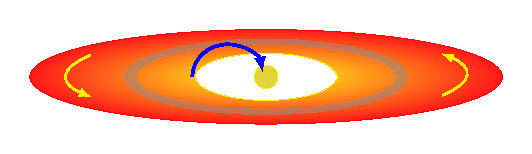
\includegraphics[width=10cm]{sketches/ctts.pdf}
\caption{Sketch of a classical T~Tauri system. \label{fig:ctts_sketch}}
\end{figure}


\subsection{Brief context of other relevant observations}
{\color{blue}(Ha for accretion, images/IFU for jets)

Examplary Xshooter spectrum [HMG: I sugest to just ask Carlo for a figure] Venuti et al. 2019?

        IFU image(s) from Takami monitoring
}
\section{Accretion}
{\color{blue}(10 pages)}
Accretion is the defining factor for young stars, it is through accretion that they build up mass, it is through accretion that they accumulate angular momentum, and it is probably through magnetic connection between disk and accretion column that at least some part of their angular momentum is lost. Once accretions stops, the mass, chemical composition, and angular momentum of a star only evolved very slowly through winds, on time scales similar to how main-sequence stars evolve.

\textbf{HMG: Very hard to write in our original order. I re-organized, so we need to adjust once we settle the order of the subsections.}
In this section, we first give an overview the physics of accretion and accretion columns (section~\ref{sect:accretionphysics}) and then we review what models and simulations have been built to study the details of the accretion process and what we can learn from that (section~\ref{sect:accretionmodels}) before we pivot to review observations of the accretion shock itself (section~\ref{sect:accretionobs}) and other supporting observational evidence (section~\ref{sect:accretionsupportingobs}).



\subsection{Observations of accretion}
\label{sect:accretionsupportingobs}
{\color{blue}           Moritz

 Observations of the magnetospheric accretion region (e.g Bouvier et al.)
 
 probably also want some Ha variability, even if we write an X-ray review. Large choice, maybe Alencar?
}

% Moritz list of citations to be put in the correct location later
TW Hya redshift plasma  38.3 ± 5.1 km s-1  2017A&A...607A..14A 
MHD modelin coal abs 2014ApJ...795L..34B 

2011A&A...526A.104C curran




\subsection{X-ray signatures of the accretion shock}
\label{sect:accretionobs}
{\color{blue}Moritz, Christian

Kastner & Brickhouse spectra, other spectra?, Argiroffi redshift? yes, Brickhouse 2012 variability,  naturepaper solar!}

The X-ray emission from cool stars on the main-sequence (MS) stars is caused by coronal activity. Young stars rotate faster and thus have more magnetic activity and thus also stronger coronal X-rays that older MS stars such as our Sun. That is way accretion signatures are hard to find in broad-band X-ray spectra and 

Using high-resolution grating spectroscopy from Chandra \citet{Kastner_2002} introduced additional diagnostics. Most importantly, the density of the emitting plasma can be determined from line ratios in the O~{\sc vii} and Ne~{\sc ix} triplets, which can be resolved into three lines with XMM-Newton or Chandra grating spectroscopy: A resonance line ($r$), an intercombination line ($i$), and a forbidden line ($f$). In collisionally excited plasma, the $f$ line is typically stronger than the $i$ line, but collisions in high-densities plasma or strong UV fields (relevant in A or B stars, but not in the lower-mass classical T Tauri stars) can excite an electron from the upper level of the $f$ line to the upper level of the $i$ line. A low $f/i$ ratio is thus a sign of high densities in the emission region, which leads to the idea that this X-ray emission originates behind the shock front of an accretion shock.

\citet{Guenther_2007} compared XMM-Newton data from TW~Hya to updated models that explicitly predicted these density-sensitive line ratios and could explain the available data of TW~Hya at the time. In this case, about two thirds of the total X-ray flux must be due to the shock, with the remaining emission coming from a stellar corona. However, deeper observations, again for TW~Hya \citep{Brickhouse_2010}, 


\subsection{Physics of accretion}
\label{sect:accretionphysics}
{\color{blue}(free-fall, accretion shock, plasma temperature, X-ray emission, etc.) [Moritz, Sabina]
Accretion sketch Hartmann et al. 2016 - we might use our own picture, too.

}

Accretion happens when mass from the circumstellar disk is transferred onto the stellar surface. In the basic model of magnetically funneled accretion, the stellar high-energy radiation ionizes the inner edge of the disk. When the stellar magnetic field connects to the inner edge of the disk, matter can flow along the field lines and impact onto the star, where a strong shock forms. The accretion column is relatively cool, but in the shock that gas is heated up to X-ray emitting temperatures. Depending on the exact location of the shock, those X-rays may or may not be visible, but the shock certainly heats the surrounding photosphere, which causes bright UV emission and an optical veiling (a strong continuum that makes phtotospheric emission lines appear weaker than in a non-accretion star.)

As the star and the disk rotate, and the magnetic field and the disk structure evolves, the accretion geometry and the accretion rate can change on time scales as short as minutes or as long as centuries; accretion can also switch off temporarily or permanently, as the star looses its disk. Despite that, many basic aspects of the accretion physics can be described in a 1D model where all mass motion happens parallel to the magnetic field. In the next few sub-sections we review some of the basic physics of accretion columns and accretion shocks. While modern models go far beyond such a simple prescription, the foundation of all accretion shock models still is to convert the graviational energy in the disk to kinetic energy of the infalling gas, which in turn gets turned into heat and radiation in the accretion shock.

\subsubsection{Free-fall velocity}
The free fall velocity $v_{\textnormal{free}}$ of material coming from an inner disk radius of $R_\mathrm{in}$ onto a star with mass $M_*$ and radius $R_*$ is
\begin{equation} 
v_{\textnormal{free}} = \sqrt{{2GM_*} \left(\frac{1}{R_*} - \frac{1}{R_\mathrm{in}}\right)} \approx 620 \sqrt{\frac{M_*}{M_\odot}}\sqrt{\frac{R_\odot}{R_*}} \frac{\textnormal{km}}{\textnormal{s}}\ \label{eqn:freefall} 
\end{equation}
where $G$ is the gravitational constant. The inner radius is typically a few stellar radii and thus $v_\textnormal{ff}$ is very close to infall from infinity.


\subsection{Calculation of shock front}
All turbulent fluxes are neglected and we only treat stationary shocks. In the shock front, ions and electrons are heated differently, but they remain strongly coupled and reach the same temperatures with in a few mean-free path lengths - a region so thin that it is justified to treat them as a single fluid. 

Somewhere along the accretion column, a shock forms when the forward ram pressure becomes comparable to the pressure of the underlying material. The shock front itself is very thin, only of the order of a few mean free paths \citep{raizerzeldovich}. Therefore it can be treated as a mathematical discontinuity described by the Rankine-Hugoniot jump-conditions \citep[][chap.~7, \S~15]{raizerzeldovich}; in the shock the super-sonic infall velocity is converted mostly into thermal energy. To simplify the numerical treatment we assume the direction of flow parallel to the magnetic field, so the Lorentz force does not influence the dynamics. Marking the state in front of the shock front by the index 0, that behind the shock by index 1, the Rankine-Hugoniot conditions become
\begin{eqnarray}
\rho_0 v_0 &=& \rho_1 v_1 \label{RH1}\\
P_0+\rho_0 v_0^2 &=& P_1+\rho_1 v_1^2 \label{RH2}\\
\frac{5 P_0}{2\rho_0}+\frac{v_0^2}{2}&=&\frac{5 P_1}{2\rho_1}+\frac{v_1^2}{2} \ ,\label{RH3}
\end{eqnarray}
where $v$ is the velocity, $\rho$ the total mass density of the gas and $P$ its pressure. 

From the jump conditions, the shocks will heat gas to a temperature
$$
kT \simeq \frac{3}{16}\mu m_p v^{2} \approx 0.3\,{\rm keV}\left(\frac{v}{500\,{\rm km/s}}\right)^{2},
\label{eqn:Tshock}
$$
where $\mu$ is the dimensionless atomic weight.

\subsubsection{Structure of the post-shock region}

In the following section we compute how the originally different kinetic temperatures of ions and electrons as well as the ionisation temperature
equilibrate and calculate the emitted X-ray spectrum.

\paragraph{Momentum balance}\label{hydrodyn}

In the post-shock region the gas emits radiation and cools down, so the energy of the gas is no longer conserved.  However, the particle number flux $j$ of ions (and atoms) 
\begin{equation}j=nv\label{j_n}\end{equation}
is conserved, where $n$ is the ion/atom number density; the electron number density is denoted by $n_{\mathrm{e}}$. The total momentum flux $j_p$ is conserved, since we ignore the momentum loss by radiation; it consists of the ion and the electron momentum as follows:
\begin{eqnarray}  
j_p&=&\mu m_{\mathrm{H}} n v^2+P \nonumber \\
   &=&\mu m_{\mathrm{H}} n v^2+nkT \label{j_p}
\end{eqnarray}
with $P$ is the thermodynamic pressure and $T$ the temperature; $m_{\mathrm{H}}$ denotes the mass of a hydrogen atom.

\paragraph{Energy balance}
\label{sect:energybalance}

Let us next consider the energy balance in the post-shock region. In general,  
\begin{equation} \label{tsminuspdvisdu} T d\Sigma -P dV=dU \end{equation}
where $\Sigma$ denotes the entropy and $U$ the internal energy of the plasma. The quantity $T d\Sigma=dQ$ denotes the heat flux through the boundaries of the system; one important component of the is the energy loss $Q_{col}$ through collisions that excite higher electronic states, which will than decay through radiation. 

Assuming that the shock location is stationary, we get $\frac{d}{dt}=\frac{\partial}{\partial t}+\frac{\partial z}{\partial t}\frac{\partial}{\partial z}=v\frac{\partial}{\partial z}$ depending on the location $z$, measured from the shock front inwards; differentiation with respect to $z$ will be indicated by $'$.
The internal energy $U$ is in this case the thermal energy $U=\frac{3}{2}kT$, the pressure $P$ can be rewritten using the equation of state. The specific volume $V$ is the inverse of the number density $V=\frac{1}{n}$. 
It is convenient to write the electron number density as \mbox{$n_{\mathrm{e}}=x_e n$,} with $x_e$ denoting the number of electrons per heavy particle.
\begin{equation}
\label{energyelec}
v\left(\frac{3}{2}x_e k T_{\mathrm{e}}\right)'+v x_e n k T_{\mathrm{e}} \left(\frac{1}{n}\right)'=-Q_{col} x_e n,
\end{equation} 

We now have $n$, $v$, and $T$ as variables and three hydrodynamic equations (\ref{j_n}, \ref{j_p}, and \ref{energyelec}), so the structure of the post-shock region can be calculated.


\subsection{Models}

\label{sect:accretionmodels}
{\color{blue}(historic evolution of models and aspects addressed by models) [Moritz, (Sabina)]

Accretion column models Lamzin 2004, Robinson & Espaillat?; C IV lines (Lamzin 2003?); accretion rates

a figure from any Romanovy work


Radiative transfer (Colombo et al. )

Laboratory experiments (e.g. Burdonov et al. 2020)
}

Early simulations follow the 1D prescription given above, which was sufficient to explain the high-energy data at the time. They show that the accretion shock produces plasma matching the observed X-ray temperatures \citep{lamzin_1998} and that the total energy in the accretion stream can be determined from fitting UV and optical spectra to determine the mass accretion rate \citep{calvet_1998}.

Using high-resolution grating spectroscopy from Chandra \citet{Kastner_2002} introduced additional diagnostics. Most importantly, the density of the emitting plasma can be determined from line ratios in the O~{\sc vii} and Ne~{\sc ix} triplets, which can be resolved into three lines with XMM-Newton or Chandra grating spectroscopy: A resonance line ($r$), an intercombination line ($i$), and a forbidden line ($f$). In collisionally excited plasma, the $f$ line is typically stronger than the $i$ line, but collisions in high-densities plasma or strong UV fields (relevant in A or B stars, but not in the lower-mass classical T Tauri stars) can excite an electron from the upper level of the $f$ line to the upper level of the $i$ line. A low $f/i$ ratio is thus a sign of high densities in the emission region, which leads to the idea that this X-ray emission originates behind the shock front of an accretion shock.

\citet{Guenther_2007} compared XMM-Newton data from TW~Hya to updated models that explicitly predicted these density-sensitive line ratios and could explain the available data of TW~Hya at the time. In this case, about two thirds of the total X-ray flux must be due to the shock, with the remaining emission coming from a stellar corona. However, deeper observations, again for TW~Hya \citep{Brickhouse_2010}, 

camer, birckouse, accretion stream, orlando

Similarly, improved models including LTE radiation transfer now show that the heated photosphere does not radiate as a simple black body in the optical and infrared \citep{Dodin_2012,Dodin_2013}, but that is also produces lines, which selectively fill in some photospheric absorption lines, possibly biasing accretion rate measurements based on optical veiling.

Shoud out to global models pf the accretion stream (romanova, etc.)

\subsection{The multi-D structure of the accretion shock}

Most observations of the structure of the accretion shock on young stars are spatially unresolved; only Doppler-imaging can at least reveal the location on the surface where the accretion shock happen. Yet, it would be very valuable to learn about the detailed 3D geometry and the time evolution of accretion shocks to interpret the unresolved data. For example, it is unclear if the accretion shocks forms deeply in the photosphere where it is hidden from view or higher up in the accretion funnel. One approach to address this problem is to perform experiments in the laboratory using a set-up where magnetic fields, densities, temperatures, and other hydrodynamical parameters are chosen to scale to the stellar case. In one example of such work, \citet{2017SciA....3E0982R} find that plasma is ejected laterally from the accretion shock and forms a shell around the infalling stream. This hot shell provides an additional absorber that reduces the shock emission that is directly observable. Recently, \citet{2020A&A...642A..38B} extended this work to accretion streams not perpendicular to the impacted surface as it might happen for accretion stream along complex magnetic field structures. They find the resulting plasma flows to be highly asymmetric and see a large amount of plasma escaping laterally from the accretion flow.  

Another approach is to look for analogous situations in our Sun, where spatially resolved data in the UV and EUV, even if not in X-rays, is available with long time coverage and high cadence. One particular event happened on June, 7$^{th}$, 2011, when parts of an erupting filament fell back into the Sun \citep{2013Sci...341..251R,2013A&A...559A.127O}. The infall speed of up to 450~km/s was comparable to free-fall accretion onto T Tauri stars, but the accretion rate was obviously much lower. Similar to the laboratory experiments, the initial infall triggered upflows, but here they shocked with later fragments causing UV emission.

Both, laboratory experiments and the solar analogy, point to a significantly more complex picture than the simple 1D accretion shock outlined in section~\ref{sect:accretionphysics}. Simulations of the accretion shock 


might explain low m rates... nh in TW hya , MHD simulations here...

\section{Jets}
 {\color{blue}        (10 pages)}
 
 

\begin{figure}[t]
% \centering

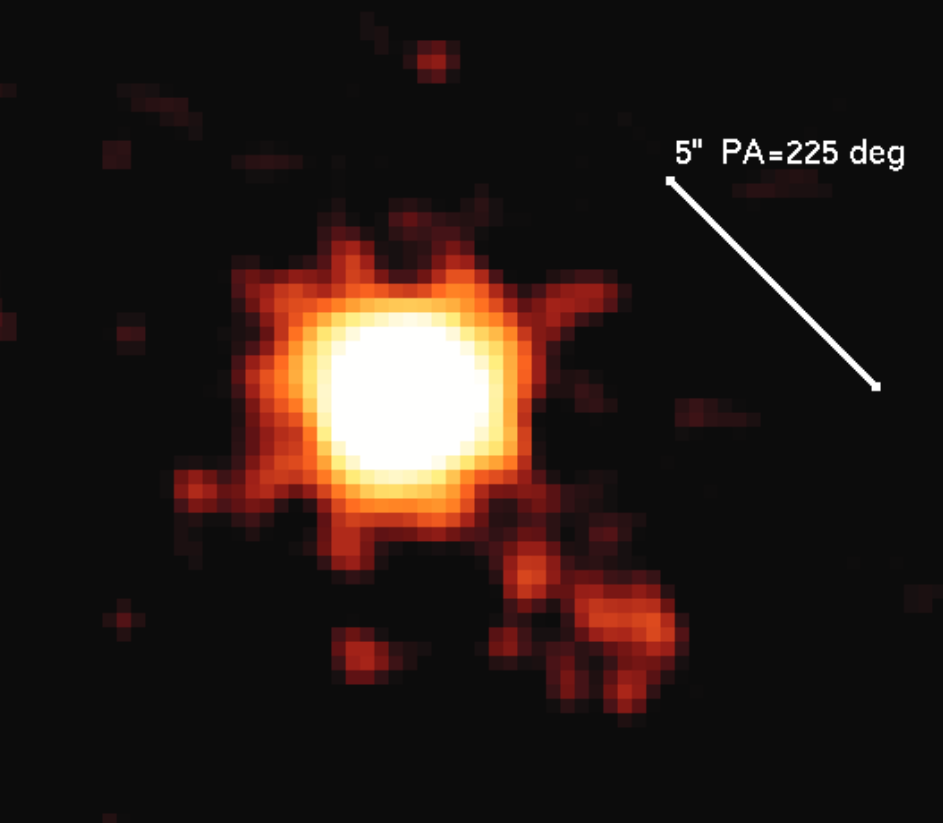
\includegraphics[width=6cm]{figs/dg_tau_X}
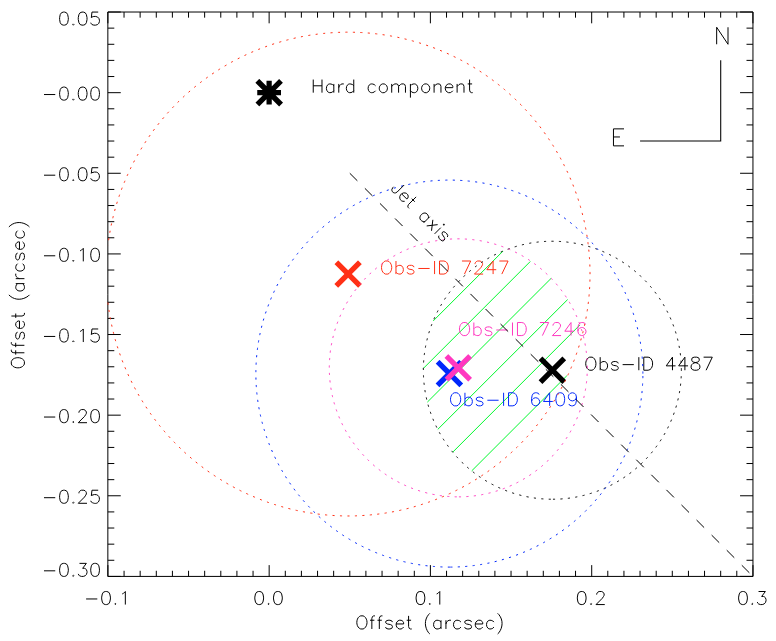
\includegraphics[width=6cm]{figs/dg_tau_offsets}

\caption{{\bf Left: } Chandra X-ray image of the DG~Tau system. From \citet{2011ASPC..448..617G}.
         {\bf Right: } Relative spatial offsets between the hard (coronal) and soft (jet) emission. From \citet{Schneider_2008}. \label{fig:dg_tau_X}}
\end{figure}

 
 A variety of mass ejection phenomena occur during the first stages of star evolution which are intimately related to the accretion process described in the previous section. In general they are presented as ejections of plasma from a young star which propagates in the ambient medium with supersonic velocities. Outflows in pre-main sequence stars (PMS) are detected in a wide range of wavelengths and they show very different morphologies, from jets to less-collimated lobes that form an extended cavity-wall. In this review section we focus on protostellar jets which are well collimated beams that in general show X-ray emission. Here we will describe the physics of jets in PMS stars, the X-ray observations and the aspects addressed by X-ray emission models.
 
\subsection{Physics of jets}
{\color{blue}(jet origin, collimation, jet velocities) [Christian, Sabina]}



\begin{figure}[t]
\centering

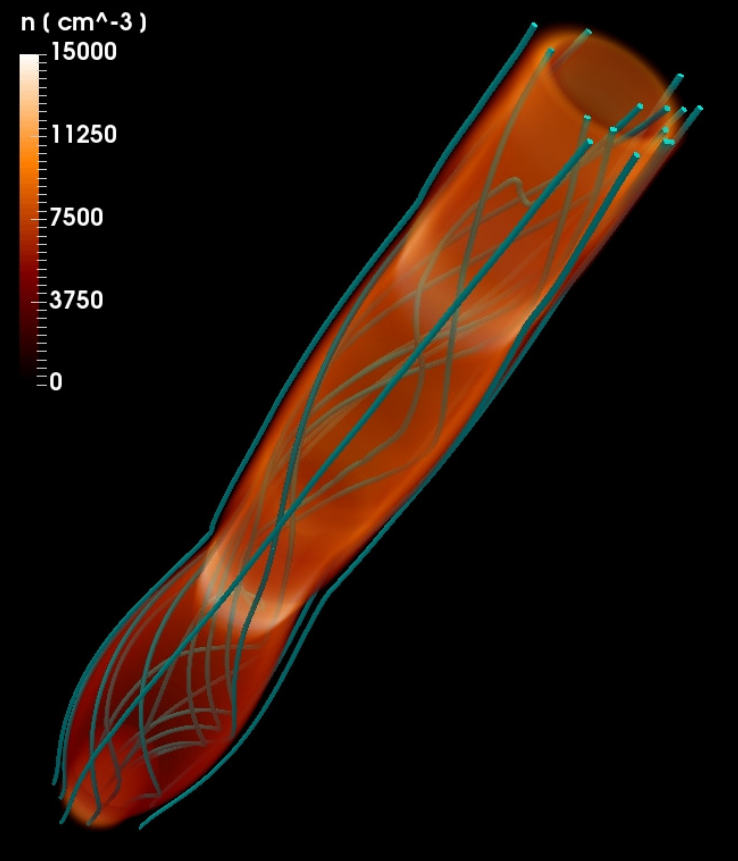
\includegraphics[height=6cm]{figs/diamond}
% % % 
%  \vspace*{-0.5cm}
 %
 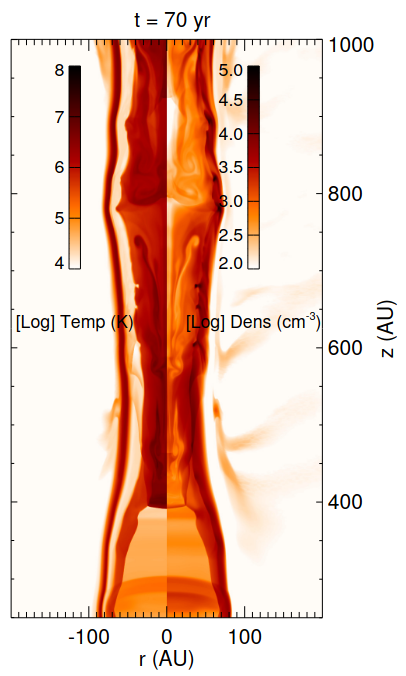
\includegraphics[height=7cm]{figs/diamond_simu}

\caption{{\bf Left: } Structure of jet and magnetic field close to the base. From \citet{Ustamujic_2016}.
         {\bf Right: }. From \citet{Ustamujic_2018}. \label{fig:jet_simu}}
\end{figure}

Sketch (suggestion?) should we make a new sketch?

Wind, outflows and jets: Bally 2016 (main components of outflows); Matt & Pudritz 2005 (accretion powered winds), Zanni & Ferreira 2013 (magnetospheric ejections)}


\subsection{X-ray jet observations}
{\color{blue}Christian

Favata HH 154, Guedel DG Tau, Schneider HH 154

Laboratory experiments  e.g. Revet et al. 2017
}
\subsection{Models of X-ray emission from jets}
{\color{blue}Sabina
3D view based on Ustamujic et al. MHD model}



\begin{figure}[t]
\centering

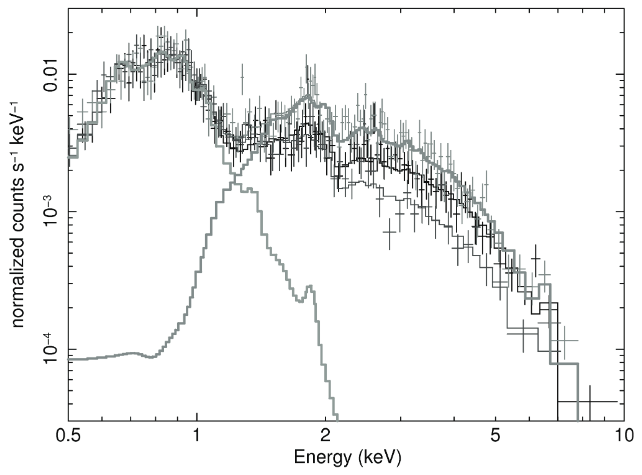
\includegraphics[height=6cm]{figs/tax}
% % % 
\caption{X-ray spectrum of DG~Tau showing the two absorber nature. From \citet{}. \label{fig:tax}}
\end{figure}



\begin{figure}[t]
\centering

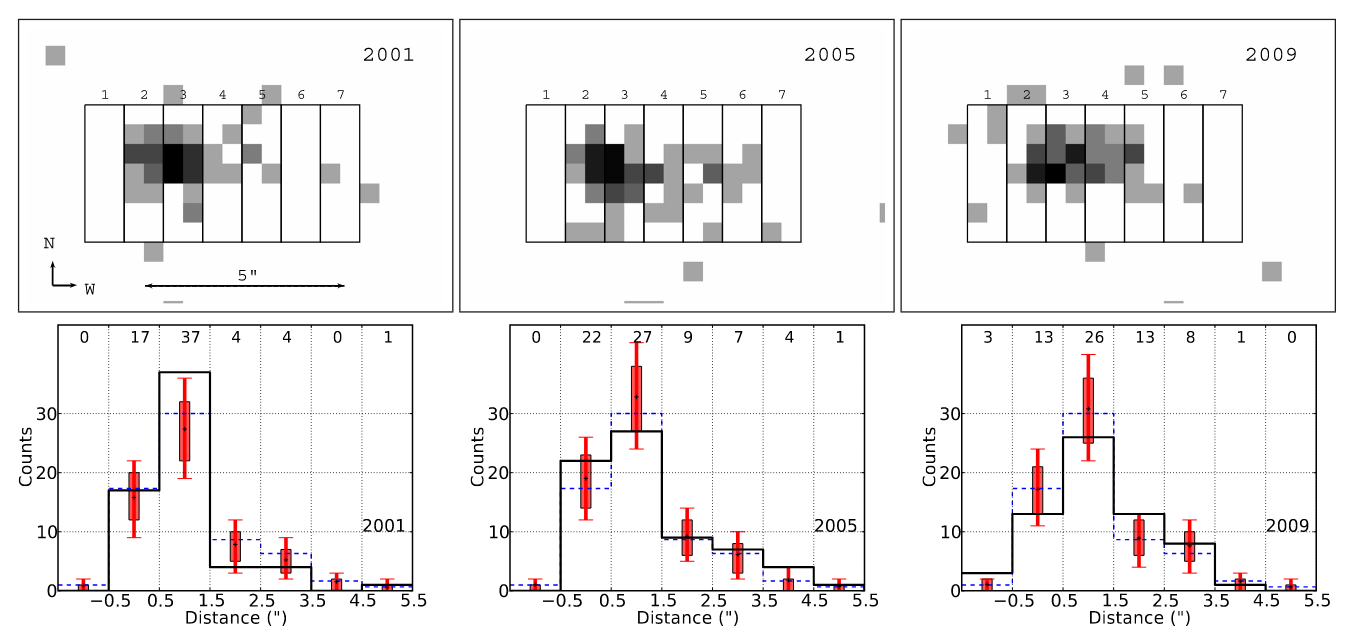
\includegraphics[height=6cm]{figs/hh154}
% % % 
\caption{Evolution of the X-ray emission from HH 154. From \citet{Schneider_2011}. \label{fig:hh154}}
\end{figure}


\begin{figure}[t]
\centering

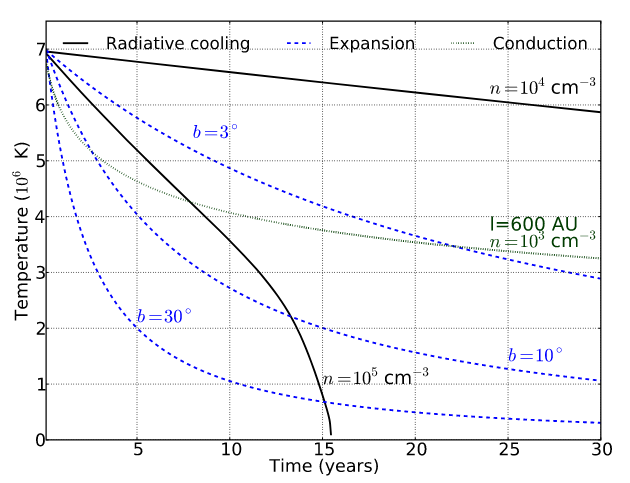
\includegraphics[height=6cm]{figs/cooling}
% % % 
\caption{Cooling of an expanding, X-ray emitting plasma. \label{fig:cooling}}
\end{figure}


{\color{blue}Sabina
Stationary X-ray emission, HH objects

Collimation by the rotating magnetic field or wind pressure

Bonito et al? (HMG: Not a big fan of the setup wit ha ``nozzle'' at the disk which then leads to the diamond shock, but they are often cited and instructuve picture)

Lab work in here, too?
}


\begin{figure}[t]
\centering

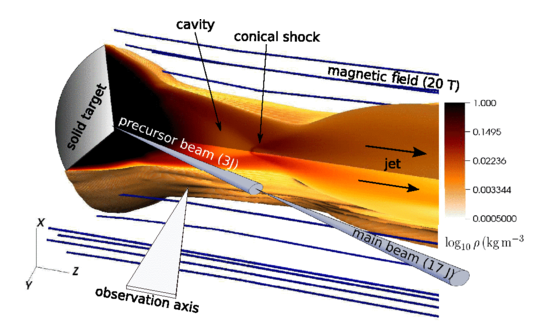
\includegraphics[height=6cm]{figs/lab}
% % % 
\caption{Lab experiment. From \citet{PhysRevLett.119.255002}. \label{fig:lab}}
\end{figure}


\subsection{Connection to other obs}
{\color{blue}Christian

UV obs (DG Tau jet), [Fe II] monitoring, Liu [Ne III]?

Jet rotation
}
\section{Outlook}
{\color{blue}(2 pages) [all]

Athena, Lynx, Arcus (figures will be new, Moritz can make for Lynx, Arcus)(?)
}


\section{Instruction - DELETE}

\vspace{0.3cm}

{\bf Key-points to have in mind}:
\begin{enumerate}
\item The {\it Handbook of X-ray and Gamma-ray Astrophysics} is aiming to publish a work of tertiary literature, which provides easily accessible, digested and established knowledge derived from primary or secondary sources in the particular field. Therefore, your contribution should be clear and concise and be a comprehensive and up-to-date overview of your topic.
\item Length of text: every chapter normally consists of about 10,000-20,000 words (excluding figures and references), which would be about 20-40 typeset pages. However, this is not a rigid rule and it is something to discuss with the Section Editors of the Section of the chapter.
\item Colored figures are welcome in any standard format (jpg, tif, ppt, gif). If possible please provide the original figure in high resolution (300 dpi minimum). {\color{red}\bf Please do not forget to obtain permission in case the figure is from a published article}. For journals like ApJ, PRD, PRL, etc. you do not need the permission if you are an author of the article of the original figures, but for most journals you need the permission even if you are the author of those figures. However, if you create a new figures with minor changes, you can claim it is a new figure and you do not need any permission.
\end{enumerate}


\vspace{0.5cm}

{\bf Submission}:

\vspace{0.1cm}

{\color{red} \bf Please submit source files, compiled pdf file of the chapter, and figure permissions through the Meteor system.}

\vspace{0.5cm}

{\bf arXiv policy}:

\vspace{0.1cm}

{Authors can post their chapter on arXiv if they wish to do it. In the comment field, please write something like ``Invited chapter for {\it Handbook of X-ray and Gamma-ray Astrophysics} (Eds. C. Bambi and A. Santangelo, Springer Singapore, expected in 2022)''. After the publication of the chapter, you may add the DOI on the arXiv page.}



\section{Cross-References \textit{(if applicable)}}
Include a list of related entries from the handbook here that may be of further interest to the readers.

% bibs will be alphametically ordered. I think that's what they want.
% if not, see: https://tex.stackexchange.com/questions/312819/problem-with-springer-bibliography-stylespbasic-natbib
\bibliographystyle{spbasic}
\bibliography{bib.bib}

\end{document}
